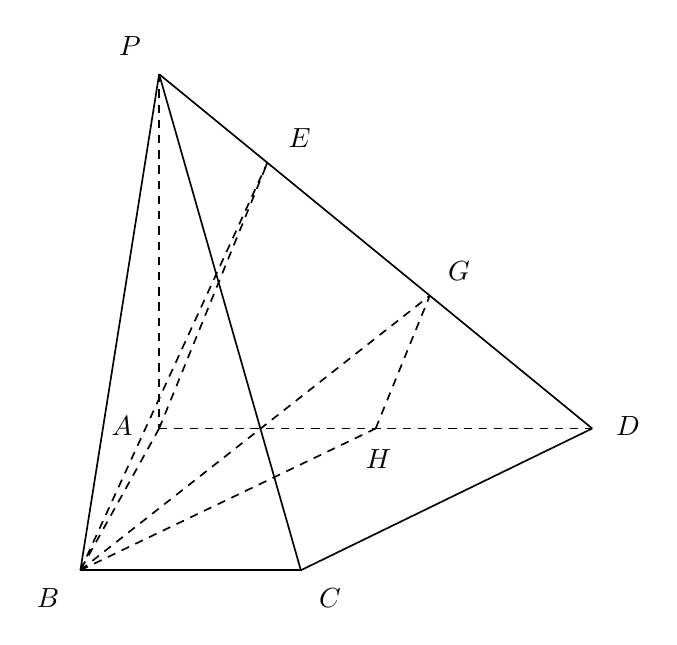
\begin{tikzpicture}[x=1cm,y=1cm,line width=.6pt,font=\normalsize,>=stealth,
  solid edge/.style={solid,line width=.6pt},
  hidden edge/.style={dashed,line width=.6pt,dash pattern=on 3pt off 2.5pt}]
\coordinate (A) at (1.0,1.0);
\coordinate (P) at (1.0,5.5);
\coordinate (D) at (6.5,1.0);
\coordinate (B) at (0.0,-0.8);
\coordinate (C) at (2.8,-0.8);
\coordinate (E) at (2.375,4.375);
\coordinate (H) at (3.75,1.0);
\coordinate (G) at (4.4375,2.6875);
\draw[hidden edge] (A)--(D);
\draw[solid edge] (B)--(C);
\draw[solid edge] (C)--(D);
\draw[hidden edge] (A)--(B);
\draw[hidden edge] (P)--(A);
\draw[solid edge] (P)--(B);
\draw[solid edge] (P)--(C);
\draw[solid edge] (P)--(D);
\draw[hidden edge] (A)--(E);
\draw[hidden edge] (B)--(E);
\draw[hidden edge] (B)--(H);
\draw[hidden edge] (H)--(G);
\draw[hidden edge] (B)--(G);
\node[above left,xshift=-3pt,yshift=3pt] at (P) {$P$};
\node[left,xshift=-6pt,yshift=1pt] at (A) {$A$};
\node[below left,xshift=-4pt,yshift=-3pt] at (B) {$B$};
\node[below right,xshift=3pt,yshift=-3pt] at (C) {$C$};
\node[right,xshift=5pt,yshift=1pt] at (D) {$D$};
\node[above right,xshift=4pt,yshift=2pt] at (E) {$E$};
\node[above right,xshift=3pt,yshift=2pt] at (G) {$G$};
\node[below,xshift=1pt,yshift=-4pt] at (H) {$H$};
\end{tikzpicture}
